\documentclass[xetex,mathserif,serif,aspectratio=169]{beamer}

\usepackage{xltxtra}
\usepackage{color}
\usepackage{url}
\usepackage{listings}
\usepackage{fontspec}
\usepackage{geometry}
\usepackage{lastpage}
\usepackage{fancyhdr}
\usepackage{amsmath}
\usepackage{amsthm}
\usepackage{amssymb}
\usepackage{blkarray}
\usepackage{multicol}
\usepackage{relsize}
\usepackage{listings}
\usepackage{xunicode}
\usepackage{xltxtra}
\usepackage{color}
\usepackage{url}
\usefonttheme[onlymath]{serif}

\definecolor{solarized@base03}{HTML}{002B36}
\definecolor{solarized@base02}{HTML}{073642}
\definecolor{solarized@base01}{HTML}{586e75}
\definecolor{solarized@base00}{HTML}{657b83}
\definecolor{solarized@base0}{HTML}{839496}
\definecolor{solarized@base1}{HTML}{93a1a1}
\definecolor{solarized@base2}{HTML}{EEE8D5}
\definecolor{solarized@base3}{HTML}{FDF6E3}
\definecolor{solarized@yellow}{HTML}{B58900}
\definecolor{solarized@orange}{HTML}{CB4B16}
\definecolor{solarized@red}{HTML}{DC322F}
\definecolor{solarized@magenta}{HTML}{D33682}
\definecolor{solarized@violet}{HTML}{6C71C4}
\definecolor{solarized@blue}{HTML}{268BD2}
\definecolor{solarized@cyan}{HTML}{2AA198}
\definecolor{solarized@green}{HTML}{859900}
\definecolor{yaleblue}{HTML}{0E4C92}

\newcommand{\yellow}[1]{\textcolor{solarized@yellow}{#1}}
\newcommand{\orange}[1]{\textcolor{solarized@orange}{#1}}
\newcommand{\red}[1]{\textcolor{solarized@red}{#1}}
\newcommand{\magenta}[1]{\textcolor{solarized@magenta}{#1}}
\newcommand{\violet}[1]{\textcolor{solarized@violet}{#1}}
\newcommand{\blue}[1]{\textcolor{solarized@blue}{#1}}
\newcommand{\cyan}[1]{\textcolor{solarized@cyan}{#1}}
\newcommand{\green}[1]{\textcolor{solarized@green}{#1}}
\newcommand{\yblue}[1]{\textcolor{yaleblue}{#1}}
\newcommand{\base}[1]{\textcolor{solarized@base01}{#1}}


\defaultfontfeatures{Mapping=tex-text}
\hypersetup{pdfstartview={FitH}}

\newcommand{\old}[1]{\fontspec[Alternate=1,Ligatures={Common}]{Hoefler Text}\fontsize{18pt}{30pt}\selectfont #1}%
\newcommand{\oldA}[1]{\fontspec[Alternate=1,Ligatures={Common, Rare}]{Hoefler Text}\fontsize{12pt}{15pt}\selectfont #1}%
\newcommand{\oldB}[1]{\fontspec[Ligatures={Common}]{Didot}\fontsize{12pt}{15pt}\color{solarized@base02}\selectfont #1}%
\newcommand{\tfont}[1]{\fontspec[Alternate=1,Ligatures={Common}]{Hoefler Text}\fontsize{12pt}{20pt}\selectfont #1}%
\newcommand{\dfont}[1]{\fontspec[Ligatures={Common}]{Didot}\fontsize{12pt}{12pt}\selectfont #1}%

\setbeamerfont{title}{family=\old}
\setbeamerfont{author}{family=\tfont}%
\setbeamerfont{frametitle}{family=\oldA}
\setbeamerfont{date}{family=\dfont}

\setbeamertemplate{navigation symbols}{}
\setbeamertemplate{footline}[text line]{%
  \parbox{0.99\linewidth}{
    \normalsize\vspace*{-24pt}\hfill{\color{solarized@base00}\insertframenumber/\inserttotalframenumber}
  }
}


\setlength{\parindent}{0pt}
\setlength{\parskip}{12pt}

\setbeamercolor{structure}{bg=solarized@base3, fg=solarized@base02}
\setbeamercolor{titlelike}{fg=solarized@cyan}
\setbeamercolor{title}{fg=solarized@blue}
\setbeamercolor{subtitle}{fg=solarized@magenta}
\setbeamercolor{alerted text}{fg=orange}
\setbeamercolor{itemize}{fg=solarized@base02}
\setbeamercolor{background canvas}{bg=solarized@base3}
\setbeamercolor{enumerate subitem}{fg=solarized@base02}

\newcommand{\minimize}{\mathop{\mathrm{minimize}}}
\newcommand{\argmin}{\mathop{\mathrm{arg\,min}}}
\newcommand{\argmax}{\mathop{\mathrm{arg\,max}}}
\newcommand{\st}{\mathop{\mathrm{subject\,\,to}}}


\usepackage[]{algorithm2e}
\usepackage{../kbordermatrix}

\begin{document}

%%%%%%%%%%%%%%%%%%%%%%%%%%%%%%%%%%%%%%%%%%%%%%%%%%%
\begin{frame}[fragile] \frametitle{} \oldB \small

\vfill

{\fontsize{0.7cm}{0cm}\selectfont Lecture 11 \\\vspace{0.2cm} Support Vector Machines III}\\\vspace{0.5cm}
24 February 2016

\vspace{2cm}

\begin{minipage}{0.6\textwidth}
Taylor B. Arnold \\
Yale Statistics \\
STAT 365/665
\end{minipage}
\hfill
\begin{minipage}{0.3\textwidth}\raggedleft

\includegraphics[scale=0.3]{../yale-logo.png}
\end{minipage}%

\end{frame}

%%%%%%%%%%%%%%%%%%%%%%%%%%%%%%%%%%%%%%%%%%%%%%%%%%%
\begin{frame}[fragile] \frametitle{} \oldB \small

Notes:
\begin{itemize}
\item Problem 3 is due this Friday
\item Problem 4 will be available on the course website later today, due next Friday
\end{itemize}

\end{frame}

%%%%%%%%%%%%%%%%%%%%%%%%%%%%%%%%%%%%%%%%%%%%%%%%%%%
\begin{frame}[fragile] \frametitle{} \oldB \small

Today
\begin{itemize}
\item Further exploration of the SVM optimization problem
\item Visualizing the effect of kernels and costs
\item A more complex example
\end{itemize}

\end{frame}

%%%%%%%%%%%%%%%%%%%%%%%%%%%%%%%%%%%%%%%%%%%%%%%%%%%
\begin{frame}[fragile] \frametitle{} \oldB \small

\textbf{\yblue{Review}}

We have the following specification of a support vector machine:
\begin{align*}
\min \quad &  \frac{1}{2} || \beta ||_2^2 \\
\text{s.t.} \quad & y_i (x_i^t \beta + \beta_0) > 1 - \xi_i, \quad i = 1, \ldots, n \\
&\xi_i > 0, \, \sum_i \xi_i \leq \text{Constant}.
\end{align*}
This defines a margin around the linear decision plane of width
$\frac{1}{|| \beta ||}$, and tries to minimize the number of errors
$\xi$ of points that are on the wrong side of the margin.

\end{frame}

%%%%%%%%%%%%%%%%%%%%%%%%%%%%%%%%%%%%%%%%%%%%%%%%%%%
\begin{frame}[fragile] \frametitle{} \oldB \small

\textbf{\yblue{Review, Dual}}

Computing the Lagrangian and calculating the dual function, we
were able to re-write this as:
\begin{align*}
\max_\alpha& \sum_i \alpha_i - \frac{1}{2} \cdot \sum_{i'} \sum_i \alpha_i \alpha_{i'} y_i y_{i'}
\blue{x_i^t x_{i'}} \\
&\text{s.t.} \quad 0 \leq \alpha_i \leq C, \quad \sum_i \alpha_i y_i = 0.
\end{align*}
Which defines a quadratic program with box constraints that can
be solved by general purpose optimization engines.

\end{frame}

%%%%%%%%%%%%%%%%%%%%%%%%%%%%%%%%%%%%%%%%%%%%%%%%%%%
\begin{frame}[fragile] \frametitle{} \oldB \small

\textbf{\yblue{Review, Kernel Trick}}

I also noted that the dual form of the problem only requires that we know the inner
product between pairs of samples of the predictor matrix. In this way, if we want to
do basis expansion, we only need to define the inner product rather than actually doing
projection into a higher space. This is called the \blue{kernel trick}.

\end{frame}

%%%%%%%%%%%%%%%%%%%%%%%%%%%%%%%%%%%%%%%%%%%%%%%%%%%
\begin{frame}[fragile] \frametitle{} \oldB \small

\textbf{\yblue{The Kernel Trick, cont.}}

The projected inner product $< h(x_i), h(x_{i'})>$ is usually
written directly as $K(x_i, x_{i'})$ for a function $K$ called
the kernel. Popular choices include:
\begin{enumerate}
\item \textbf{Linear:} $K(x, x') = <x, x'>$
\item \textbf{Polynomial:} $K(x, x') = (1 + <x, x'>)^d$
\item \textbf{Radial:}  $K(x, x') = exp(- \gamma || x - x' ||^2)$
\item \textbf{Sigmoid:}  $K(x, x') = tanh(\kappa_1 <x, x'> + \kappa_2)$
\end{enumerate}
Notice that these all require approximately the same effort to calculate as
the linear kernel.

\end{frame}

%%%%%%%%%%%%%%%%%%%%%%%%%%%%%%%%%%%%%%%%%%%%%%%%%%%
\begin{frame}[fragile] \frametitle{} \oldB \small

\textbf{\yblue{Review, Representation}}

One side result of the dual calculation also showed us that the
vector $\beta$ can be written as a weighted sum of the inputs $x_i$:
\begin{align*}
\beta &= \sum_i \alpha_i y_i x_i
\end{align*}
This is particularly useful when used in conjunction with the kernel
trick, where we instead have that:
\begin{align*}
\beta &= \sum_i \alpha_i y_i h(x_i)
\end{align*}

\end{frame}

%%%%%%%%%%%%%%%%%%%%%%%%%%%%%%%%%%%%%%%%%%%%%%%%%%%
\begin{frame}[fragile] \frametitle{} \oldB \small

\textbf{\yblue{Review, Representation}}

Now if we want to estimate $h(x_k)^t \beta$ in order to do prediction,
we again do not need to project into a higher dimensional space by
can just use:
\begin{align*}
h(x_k)^t \beta &= \sum_i \alpha_i y_i h(x_k)^t h(x_i) \\
&= \sum_i \alpha_i y_i K(x_k, x_i)
\end{align*}
For this reason most support vector machine implementation usual
store $\alpha$ or $\alpha \cdot y$ rather than $\beta$ itself
as this generalizes better to the kernel case.

\end{frame}

%%%%%%%%%%%%%%%%%%%%%%%%%%%%%%%%%%%%%%%%%%%%%%%%%%%
\begin{frame}[fragile] \frametitle{} \oldB \small

\textbf{\yblue{Rethinking the primal problem}}

Let's return for a moment to the original primal problem we
constructed:
\begin{align*}
\min \quad &  \frac{1}{2} || \beta ||_2^2 + C \cdot \sum_i \xi_i \\
\text{s.t.} \quad & y_i (x_i^t \beta + \beta_0) > 1 - \xi_i, \quad \xi_i > 0, \quad i = 1, \ldots, n.
\end{align*}
Notice that we will have either
\begin{align*}
\xi_i = 1 - y_i (x_i^t \beta + \beta_0) \quad \text{or} \quad \xi_i = 0
\end{align*}
As otherwise, we could decrease $\xi_i$ further and improve the objective
function without breaking the constraints. A commonly used notation to
specify this is called the positive part, denoted by a plus sign ($+$)
as a subscript:
\begin{align*}
\xi_i = \left[ 1 - y_i (x_i^t \beta + \beta_0) \right]_{+}.
\end{align*}

\end{frame}

%%%%%%%%%%%%%%%%%%%%%%%%%%%%%%%%%%%%%%%%%%%%%%%%%%%
\begin{frame}[fragile] \frametitle{} \oldB \small

\textbf{\yblue{Rethinking the primal problem, cont.}}

We can actually substitute this directly into the primal problem to
obtain an unconstrained form of the primal problem:
\begin{align*}
\min_\beta \quad &  \frac{1}{2} || \beta ||_2^2 + C \cdot \sum_i \left[ 1 - y_i (x_i^t \beta + \beta_0) \right]_{+}
\end{align*}
Making the substitution $\lambda = \frac{1}{2C}$, this becomes:
\begin{align*}
\min_\beta \quad & \sum_i \left[ 1 - y_i (x_i^t \beta + \beta_0) \right]_{+} + \lambda || \beta ||_2^2
\end{align*}
Which looks strikingly similar to ridge regression, but with the sum of
squares replaced with a different measurement of goodness of fit.

\end{frame}

%%%%%%%%%%%%%%%%%%%%%%%%%%%%%%%%%%%%%%%%%%%%%%%%%%%
\begin{frame}[fragile] \frametitle{} \oldB \small

\textbf{\yblue{Rethinking the primal problem}}

The value $\left[ 1 - y_i (x_i^t \beta + \beta_0) \right]_{+}$ is called
the \blue{hinge loss}. It behaves similarly in spirit to, still importantly
different from, squared error or binomial deviance.

\end{frame}

%%%%%%%%%%%%%%%%%%%%%%%%%%%%%%%%%%%%%%%%%%%%%%%%%%%
\begin{frame}[fragile] \frametitle{} \oldB \small

\textbf{\yblue{Penalized estimators}}

Using $f(x)$ to represent $X \beta + \beta_0$, we can write
linear regression as either:
\begin{align*}
[1 - y f(x)]^2   &+ \lambda \cdot || \beta ||_2^2 \\
[f(x) - y]^2     &+ \lambda \cdot || \beta ||_2^2 \\
\end{align*}
Logistic regression as:
\begin{align*}
\log[1 + e^{-y f(x)}]   &+ \lambda \cdot || \beta ||_2^2
\end{align*}
And support vector machines as:
\begin{align*}
[1 - y f(x)]_{+} &+ \lambda \cdot || \beta ||_2^2 \\
\end{align*}

\end{frame}

%%%%%%%%%%%%%%%%%%%%%%%%%%%%%%%%%%%%%%%%%%%%%%%%%%%
\begin{frame}[fragile] \frametitle{} \oldB \small

\begin{center}
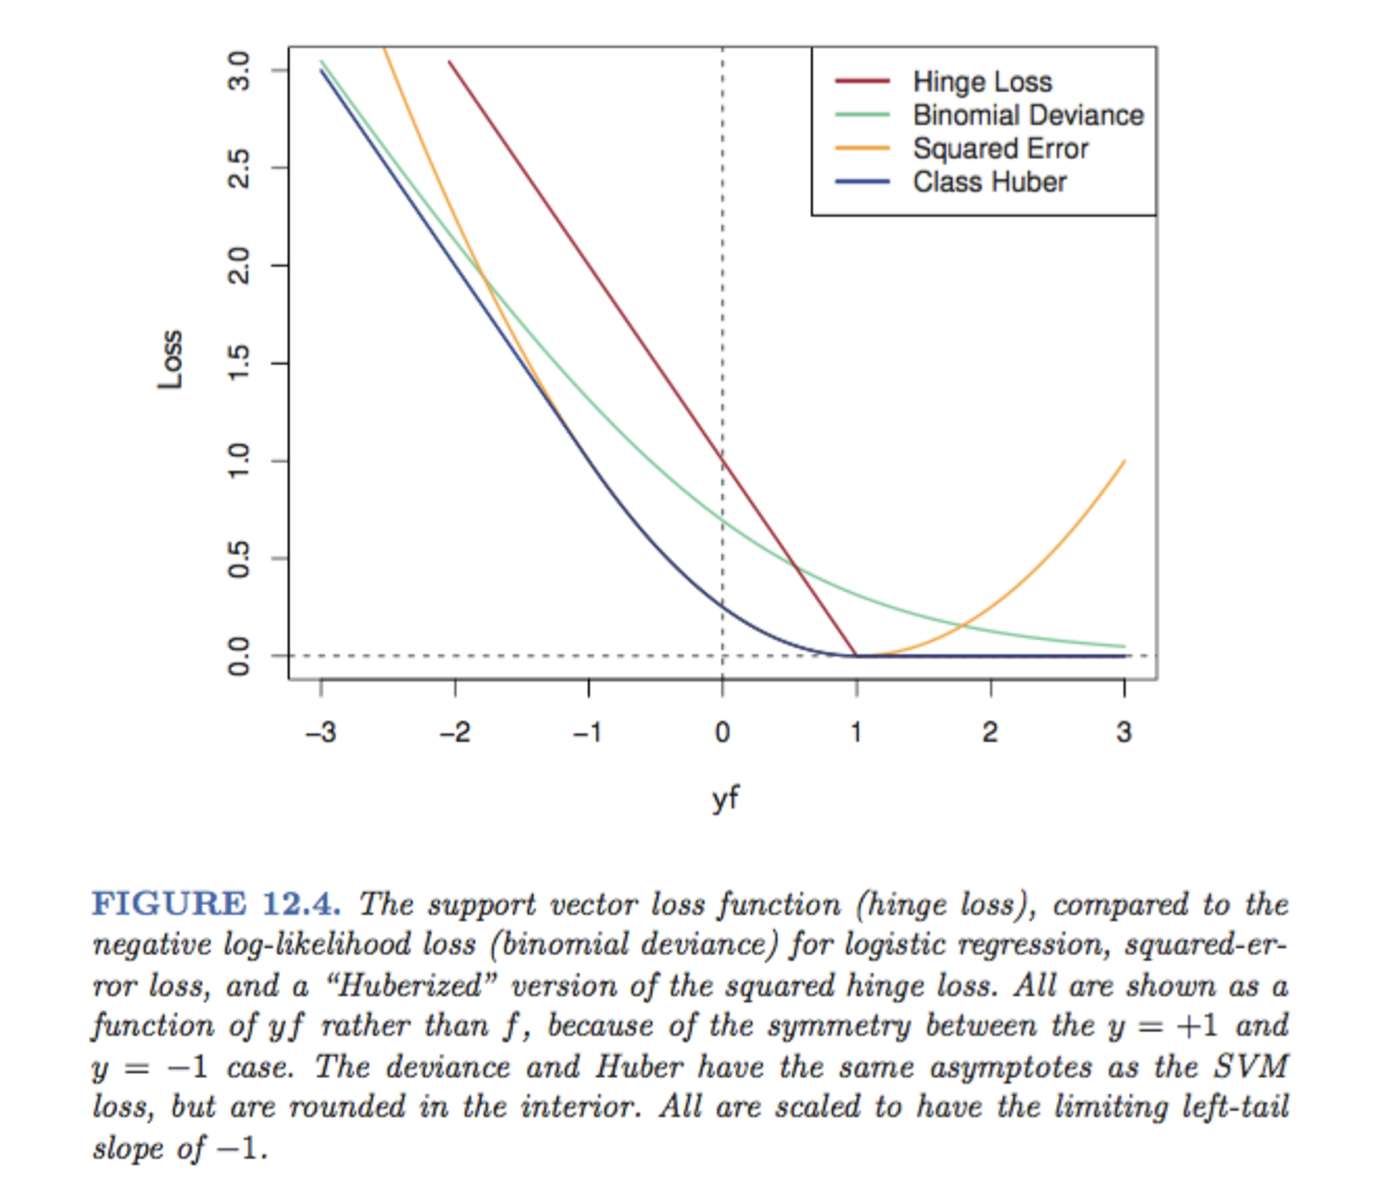
\includegraphics[height=0.7\textheight]{img/lossChoice.pdf}
\end{center}

\end{frame}

%%%%%%%%%%%%%%%%%%%%%%%%%%%%%%%%%%%%%%%%%%%%%%%%%%%
\begin{frame}[fragile] \frametitle{} \oldB \small

\textbf{\yblue{Kernels and the primal problem}}

The details go beyond the technical background I have assumed
for this course, but it is possible to rewrite this unconstrained
primal problem using the kernel trick as well:
\begin{align*}
\min_f \quad & \sum_i \left[ 1 - y_i f(x_i) \right]_{+} + \lambda ||f ||_H^2
\end{align*}
For a suitably chosen norm $|| \cdot ||_H$.

\end{frame}

%%%%%%%%%%%%%%%%%%%%%%%%%%%%%%%%%%%%%%%%%%%%%%%%%%%
\begin{frame}[fragile] \frametitle{} \oldB \small

\textbf{\yblue{The actual optimization}}

We now have two formulations for solving support vector machines:
the unconstrained primal problem given as a penalized estimator or
the box-constrained dual problem. These can than be solved by
applying a number of standard optimization techniques.

Historically, the dual formulation had been more popular because
it was obvious how to deal with kernels and the box-constraints
were easier to deal with than the constraints in the unmodified
primal problem.

However, with the reformulation of the primal problem as a penalized
unconstrained optimization objective, most new work is done on solving
the primal problem directly.

\end{frame}


%%%%%%%%%%%%%%%%%%%%%%%%%%%%%%%%%%%%%%%%%%%%%%%%%%%
\begin{frame}[fragile] \frametitle{} \oldB \small

\textbf{\yblue{The actual optimization, cont.}}

A well-written summary of recent advances that does not
require extensive background knowledge is the following
unpublished manuscript:

\begin{quote}
A. K. Menon. Large-scale support vector machines: algorithms and theory. Research Exam, University of California, San Diego, 2009. \url{https://cseweb.ucsd.edu/~akmenon/ResearchExam.pdf}
\end{quote}

\end{frame}


%%%%%%%%%%%%%%%%%%%%%%%%%%%%%%%%%%%%%%%%%%%%%%%%%%%
\begin{frame}[fragile] \frametitle{} \oldB \small

\begin{center}
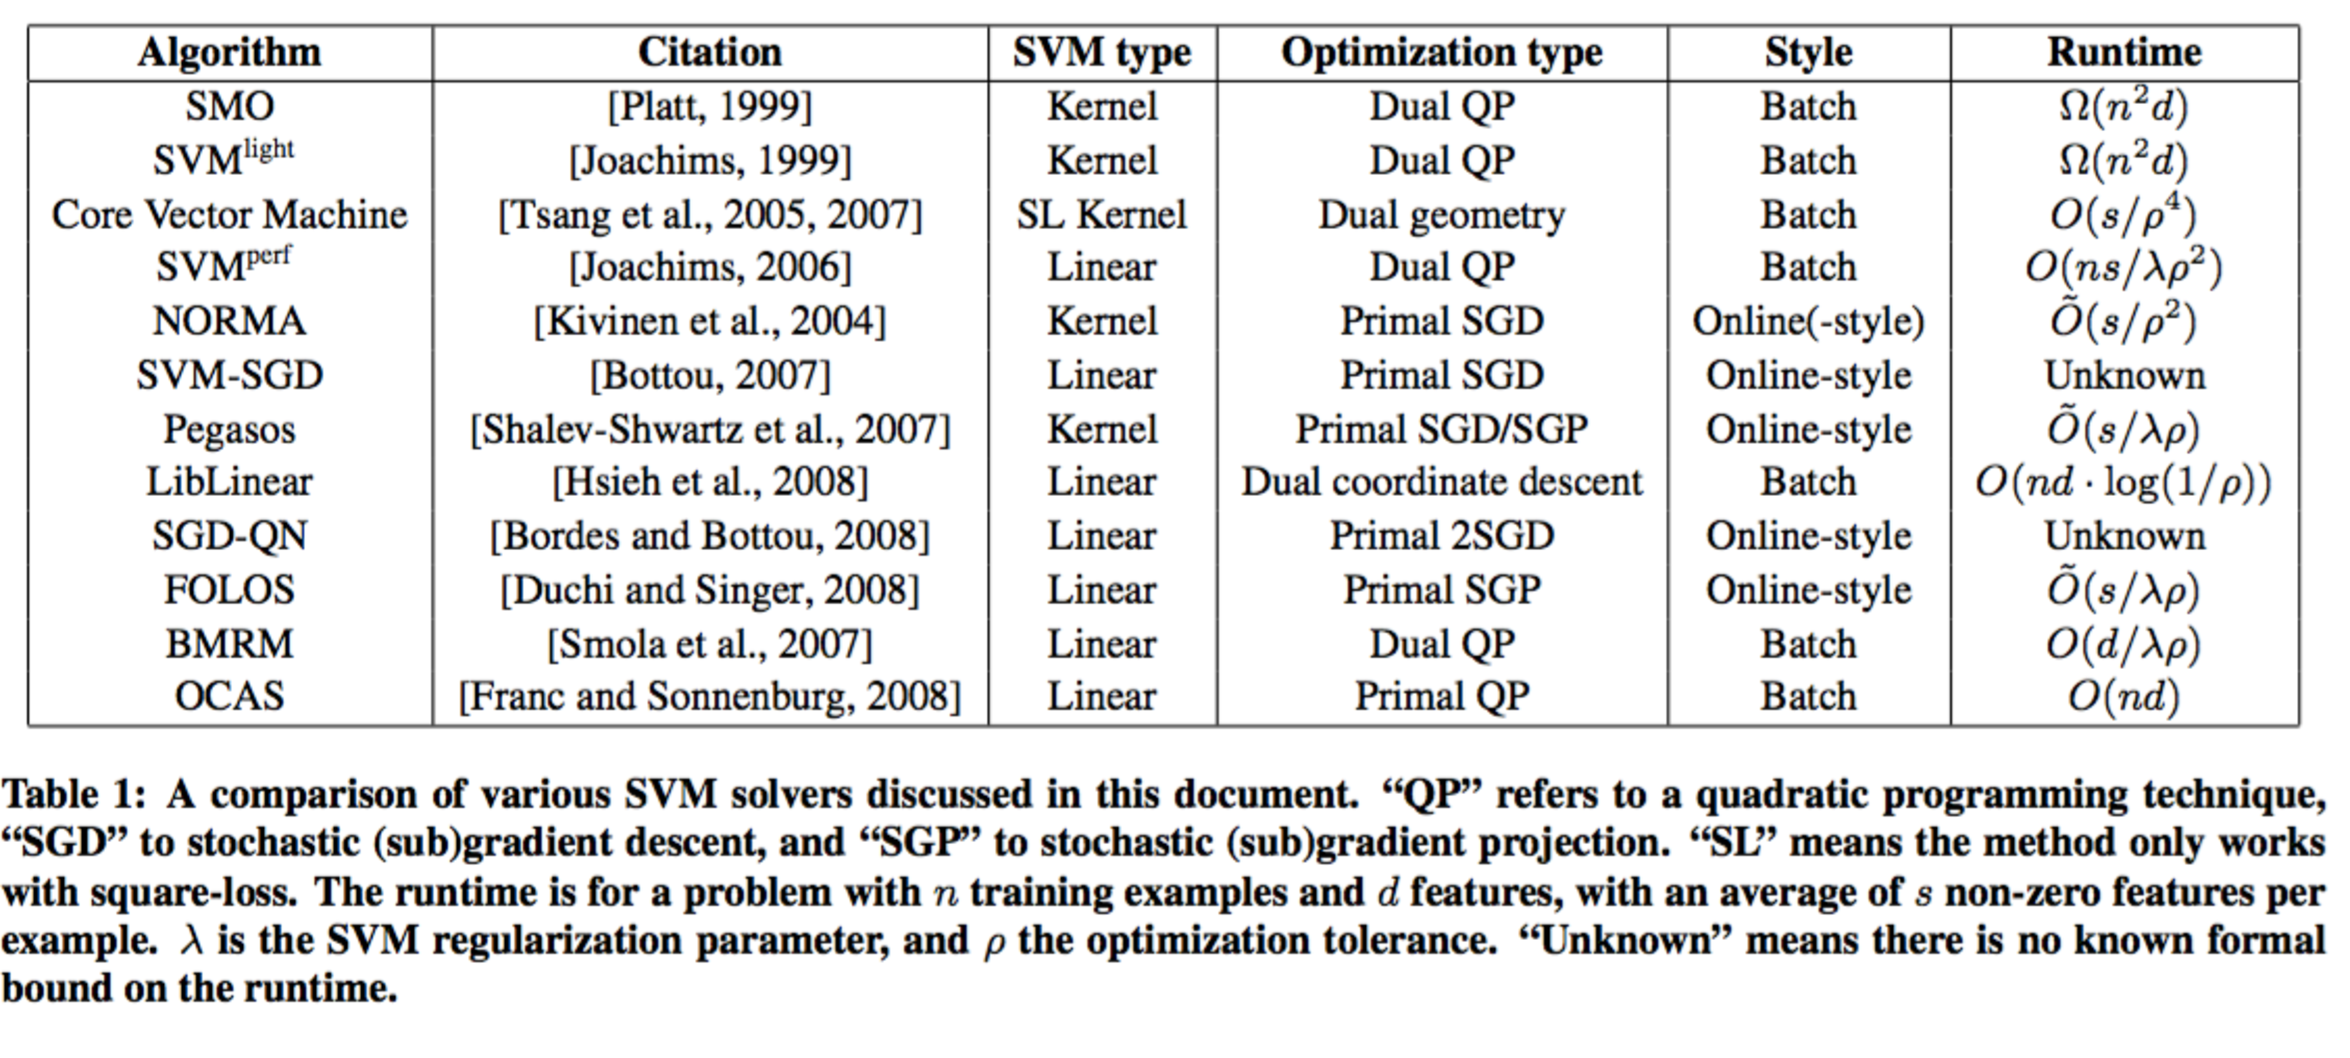
\includegraphics[width=0.7\textwidth]{img/methodCompare.pdf}
\end{center}

\end{frame}

%%%%%%%%%%%%%%%%%%%%%%%%%%%%%%%%%%%%%%%%%%%%%%%%%%%
\begin{frame}[fragile] \frametitle{} \oldB \small

\textbf{\yblue{Primal and Dual: Final Thoughts}}

In terms of the understanding support vector machines, both
formulations of the problem are quite important.

The dual
brings to light the representation of the support vector
machine as a weighted combination of a set of support vectors.
It illustrates exactly what properties make a good support
vector (dissimilar to other vectors with the same class; similar
to those with different classes). It also shows one way of
comparing and contrasting it with logistic regression.

The primal problem shows an entirely different way of comparing
logistic regression with support vector machines. It also
more clearly illustrates the role of the constant $C$ in
tuning the final model. The primal also serves as the motivation
for important modifications such as replacing the hinge loss
with a huberized variant.

\end{frame}


\end{document}











